% !TEX root = main.tex
\documentclass[10pt, a4paper]{article}

% ── Packages ──────────────────────────────────────────────────────────────────
\usepackage[
  top=0.3in, bottom=0.3in,
  left=0.45in, right=0.45in
]{geometry}
\usepackage[dvipsnames]{xcolor}
\usepackage{hyperref}
\usepackage{graphicx}
\usepackage{titlesec}
\usepackage{enumitem}
\usepackage{array}
\usepackage{tabularx}
\usepackage{parskip}

% ── Hyperlink styling ─────────────────────────────────────────────────────────
\hypersetup{
  colorlinks=true,
  urlcolor=black,
  linkcolor=black
}

\pagestyle{empty}

% Section formatting
\titleformat{\section}
  {\normalsize\bfseries}
  {}{0em}{\MakeUppercase}
  [\vspace{-6pt}\rule{\linewidth}{0.5pt}]

\titlespacing{\section}{0pt}{6pt}{2pt}

\setlist[itemize]{noitemsep, topsep=0pt, partopsep=0pt, parsep=0pt, leftmargin=1.2em, itemsep=0pt}

\setlength{\parindent}{0pt}
\setlength{\parskip}{0pt}

% Set base font size slightly larger than 10pt default
\fontsize{10.5}{13.5}\selectfont

% ══════════════════════════════════════════════════════════════════════════════
\begin{document}

% ── HEADER ────────────────────────────────────────────────────────────────────
\noindent
\begin{minipage}[c]{0.48\textwidth}
  \raggedright
  {\fontsize{24}{28}\selectfont \textbf{YOUR NAME}}\par
  \vspace{2pt}
  {\large\itshape\color{gray} Software Engineer}\par
\end{minipage}%
\hfill
\begin{minipage}[c]{0.36\textwidth}
  \raggedleft
  \begin{minipage}[c]{0.68\linewidth}
    \raggedleft
    {\small\itshape\color{gray}
      \href{mailto:your.email@example.com}{your.email@example.com}\\[3pt]
      +91\,00000\,85302\\[3pt]
      \href{https://linkedin.com/in/your-linkedin}{linkedin.com/in/your-linkedin}\\[3pt]
      \href{https://github.com/your-github}{github.com/your-github}\\
    }
  \end{minipage}%
  \hspace{0.1pt}
\begin{minipage}[c]{0.26\linewidth}
    \raggedleft
    \fboxsep=2pt\fboxrule=0.5pt
    \fbox{%
      \IfFileExists{../../assets/profile-photo.jpg}{%
        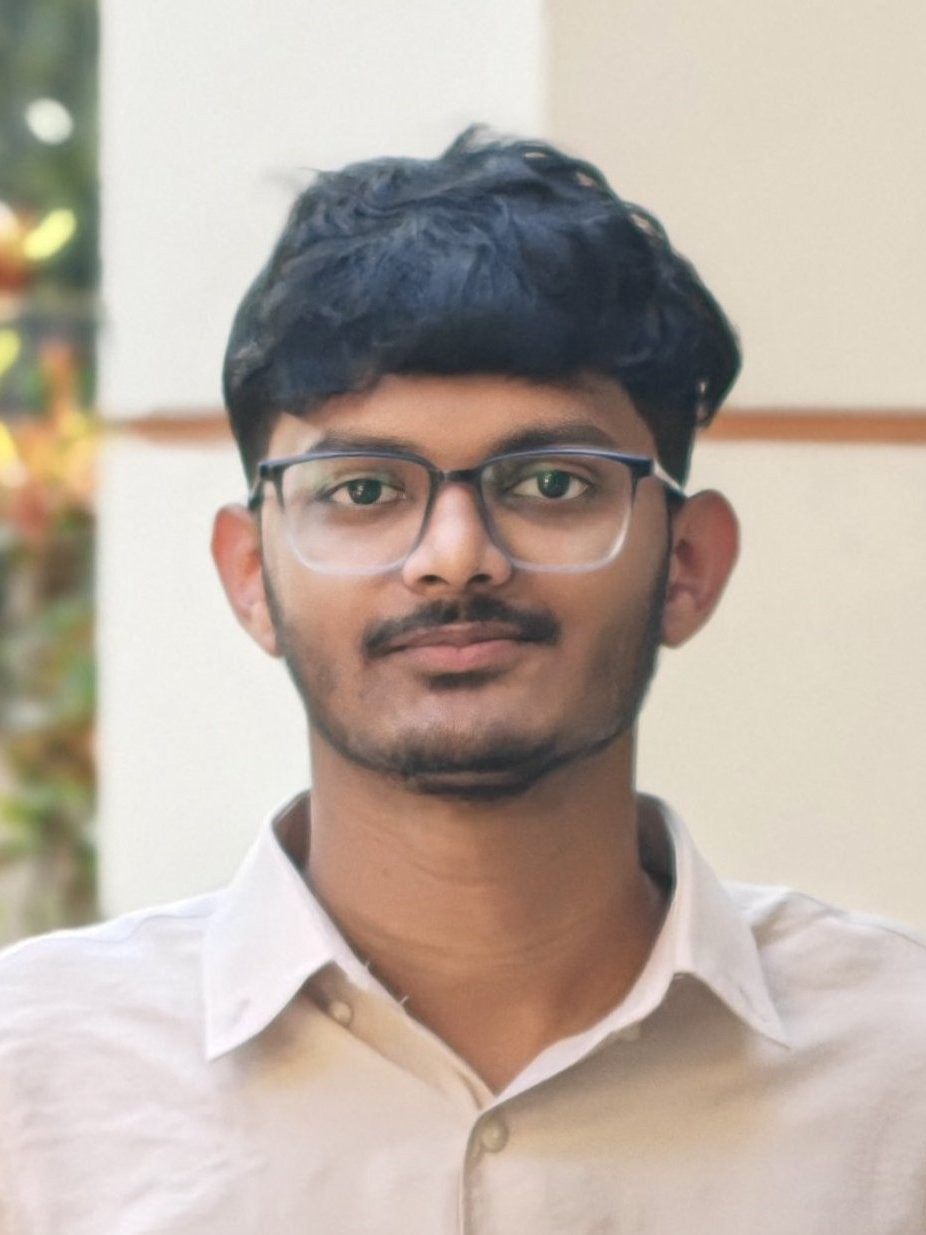
\includegraphics[height=0.75in,keepaspectratio]{../../assets/profile-photo.jpg}}{%
      \IfFileExists{../../assets/profile-photo.png}{%
        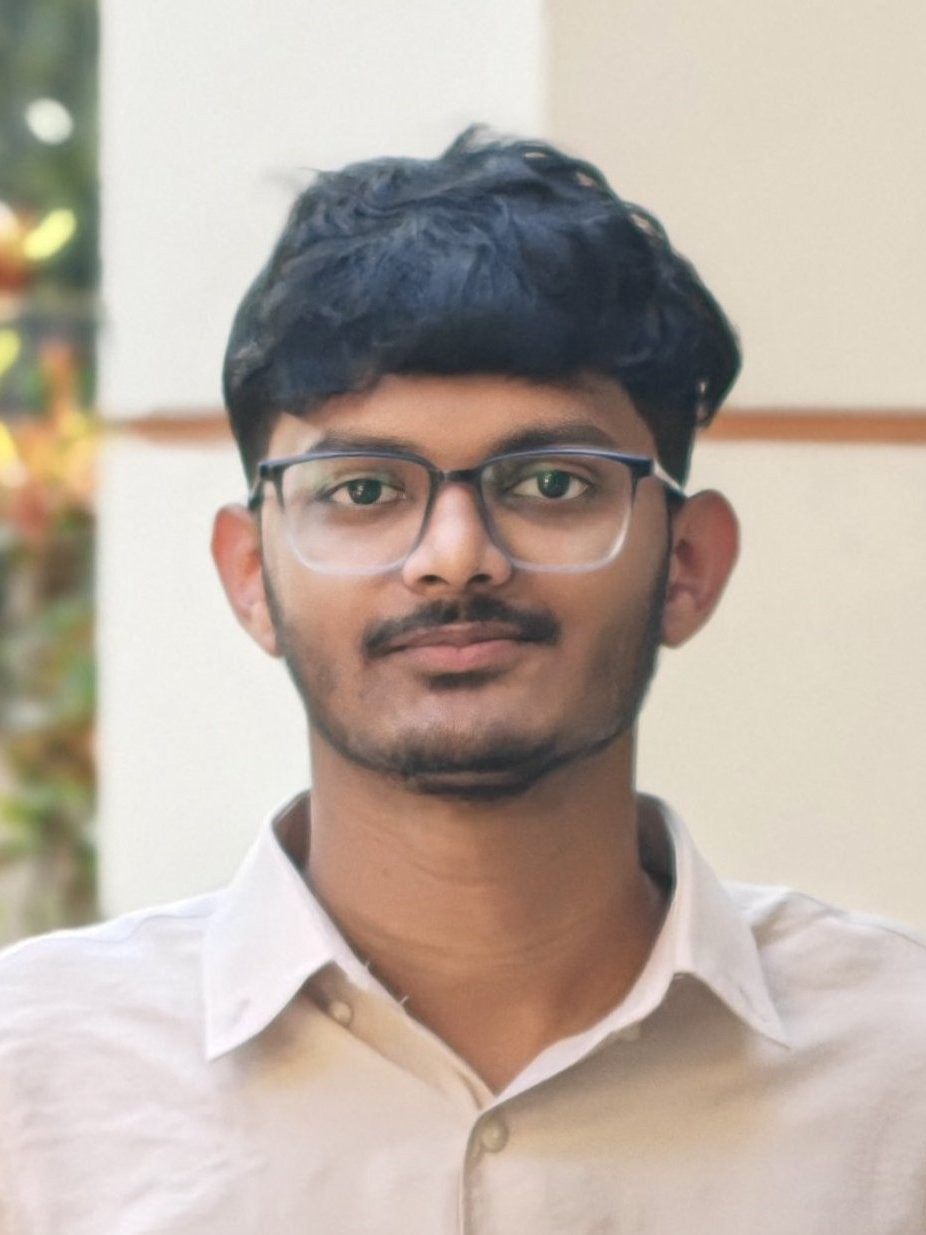
\includegraphics[height=0.75in,keepaspectratio]{../../assets/profile-photo.png}}{%
      \IfFileExists{../../assets/photo.jpg}{%
        \includegraphics[height=0.75in,keepaspectratio]{../../assets/photo.jpg}}{%
      \IfFileExists{../../assets/photo.png}{%
        \includegraphics[height=0.75in,keepaspectratio]{../../assets/photo.png}}{}}}}%
    }%
  \end{minipage}
\end{minipage}


% ── YOUR RESUME CONTENT GOES BELOW ───────────────────────────────────────────
\section*{Professional Summary}

Software Engineer with experience in backend systems, scalable applications, and real-time systems. Proficient in Python, JavaScript, and modern development frameworks, with additional experience in performance-oriented system design.

%------------------------------------------------------------
% TECHNICAL SKILLS
%------------------------------------------------------------
\section*{Skills}

\renewcommand{\arraystretch}{1.0}
\begin{tabular}{@{} >{\bfseries}p{3.8cm} p{13cm} @{}}
Languages           & Python, Java, C, JavaScript, Go, Rust \\
Web Development     & HTML, CSS, React.js, Node.js, Next.js, PHP \\
Frameworks          & Flask, Django, Express.js, Tauri, Wails, Flutter, Firebase \\
Databases           & MongoDB, MySQL, Supabase \\
Developer Tools     & Git, GitHub, Docker, Postman, REST APIs \\
Deployment          & Netlify, Vercel, Render, DigitalOcean, Cloudflare, Heroku \\
Operating Systems   & Linux, Windows \\
\end{tabular}

%------------------------------------------------------------
% PROJECTS
%------------------------------------------------------------
\section*{Projects}

\textbf{AI-Based Smart Traffic System Using Computer Vision} \hfill \textit{Python, YOLO, Flask \quad Jan 2025}
\begin{itemize}
\item Architected a YOLO-v8 detection pipeline achieving 94\% accuracy across varied traffic conditions.
\item Optimized simulated intersection throughput by 25\% via adaptive signal control algorithms.
\item Engineered low-latency model inference for real-time edge deployment and scene analysis with less than 200ms latency.
\end{itemize}

\vspace{1.5pt}

\textbf{Certificate Generator and Verification System} \hfill \textit{Node.js, Firebase, EJS, Tailwind \quad Dec 2024} \quad \href{https://github.com/your-github/advanced-certificate-generator}{GitHub}
\begin{itemize}
\item Automated high-throughput certificate generation for 1,000+ records per batch, reducing manual effort by 90\%.
\item Engineered a secure QR-based verification system enabling instant credential validation.
\item Developed an interactive canvas editor supporting dynamic layouts and reusable template components.
\end{itemize}

\vspace{1.5pt}

\textbf{IRRIGO -- Smart Irrigation Platform} \hfill \textit{Next.js, Flask, Python, REST APIs \quad Oct 2024}
\begin{itemize}
\item Developed an AI-assisted irrigation platform integrating satellite and weather data for precision scheduling.
\item Optimized agricultural water usage by \textasciitilde20\% through data-driven analysis of 50+ farm scenarios.
\item Architected a full-stack analytics dashboard for real-time monitoring and environmental telemetry.
\end{itemize}

\vspace{1.5pt}

\textbf{DroidOps -- Android Device Management GUI} \hfill \textit{Tauri, React, Rust, TypeScript \quad Dec 2025} \quad \href{https://github.com/your-github/droidops}{GitHub}
\begin{itemize}
\item Engineered a native Rust/Tauri desktop GUI for ADB, improving process execution efficiency by 40\%.
\item Leveraged Rust's memory safety and concurrency model to handle multi-device synchronization.
\item Streamlined device lifecycle management through batch processing features and optimized shell access.
\end{itemize}

\vspace{3pt}

\textbf{GlyphDeck -- Desktop Font Manager} \hfill \textit{Go, TypeScript, Wails \quad Nov 2025} \quad \href{https://github.com/your-github/GlyphDeck}{GitHub}
\begin{itemize}
\item Architected a high-performance Go application indexing 1,200+ fonts with sub-500ms retrieval latency.
\item Optimized system overhead to achieve a lightweight 25MB native executable using the Wails framework.
\item Enhanced user productivity by 40\% through optimized search algorithms and efficient metadata parsing.
\end{itemize}

%------------------------------------------------------------
% EDUCATION
%------------------------------------------------------------
\section*{Education}

\textbf{B.Tech in Computer Science and Engineering} \hfill \textbf{2022 -- 2026}\\
Mar Baselios Christian College of Engineering and Technology, Kuttikkanam \hfill APJ Abdul Kalam Technological University

%------------------------------------------------------------
% CERTIFICATIONS
%------------------------------------------------------------
\section*{Certifications}

\renewcommand{\arraystretch}{1.0}
\begin{tabular}{@{} p{7.8cm} p{6.5cm} p{2.5cm} @{}}
\textbf{Certificate}                  & \textbf{Issuer}              & \textbf{Year} \\[1pt]
Programming with Python               & Python Institute OpenEDG   & 2024 \\
Python for Data Science               & NPTEL -- IIT Madras          & 2024 \\
JavaScript Foundations Professional   & Mozilla                      & Jul 2025 \\
Amazon API Gateway for Serverless     & AWS Training                 & Jun 2025 \\
Ubuntu Linux Professional Certificate & Canonical                    & Nov 2025 \\
\end{tabular}

%------------------------------------------------------------
% ACHIEVEMENTS
%------------------------------------------------------------
\section*{Achievements}

\begin{tabular}{@{} p{9.5cm} p{8cm} @{}}
Galactic Problem Solver              & NASA Space Apps Challenge 2024 \\
Global Connection Recognition        & NASA Space Apps Challenge 2025 \\
Global Nominee                       & NASA Space Apps Challenge 2025 \\
\end{tabular}

%------------------------------------------------------------
% INTERESTS & LANGUAGES
%------------------------------------------------------------
\section*{Additional Information}

\begin{tabular}{@{} >{\bfseries}p{3.8cm} p{13cm} @{}}
Areas of Interest & Software Development, Full Stack Development, Data Structures, Algorithms, Object-Oriented Programming, API Development, Database Systems, Software Engineering \\
Languages         & English Professional, Malayalam Native \\
\end{tabular}

\end{document}